			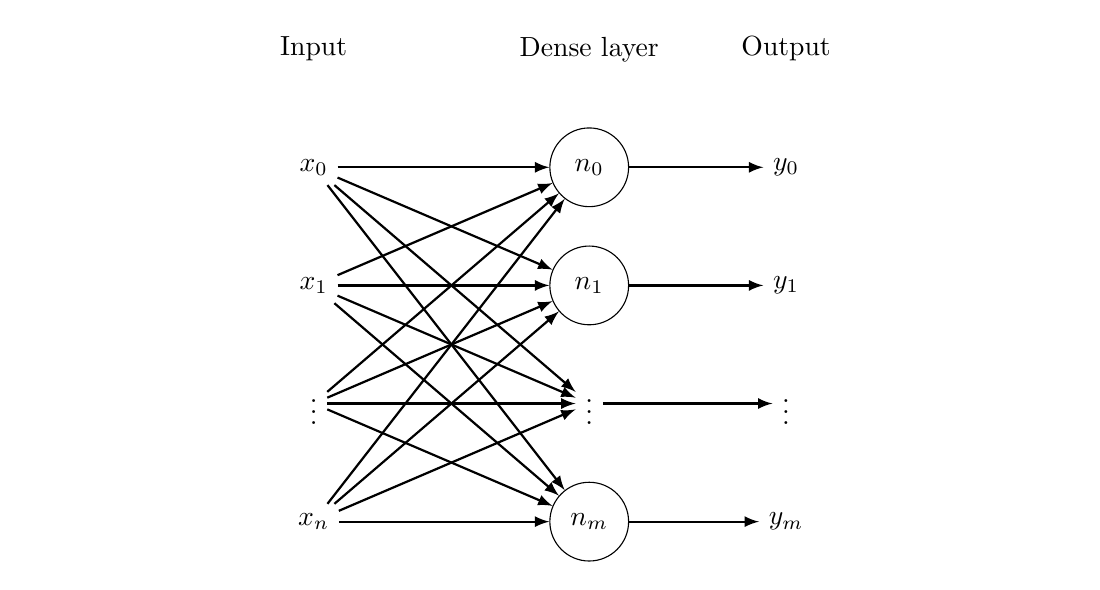
\begin{tikzpicture}[
			cell/.style={
				rectangle, 
				rounded corners=2mm, 
				draw,
				very thick,
				align=center,
			},
			ArrowC1/.style={% Arrows with rounded corners
				rounded corners=.25cm,
				thick,
			},
			]
				% input
				\node[align=center, text width=20em] (ins) at (0,6) {Input};
				\node (x0) at (0,4.5) {$x_0$};
				\node (x1) at (0,3) {$x_1$};
				\node (x) at (0,1.5) {$\vdots$};
				\node (xn) at (0,0) {$x_n$};
				% dense layer
				\node[align=center, text width=20em] (ins) at (3.5,6) {Dense layer};
				\node[draw, circle, minimum size=1cm] (n0) at (3.5,4.5) {$n_0$};
				\node[draw, circle, minimum size=1cm] (n1) at (3.5,3) {$n_1$};
				\node (n) at (3.5,1.5) {$\vdots$};
				\node[draw, circle, minimum size=1cm] (nm) at (3.5,0) {$n_m$};
				
				% output
				\node[align=center, text width=20em] (ins) at (6,6) {Output};
				\node (y0) at (6,4.5) {$y_0$};
				\node (y1) at (6,3) {$y_1$};
				\node (y) at (6,1.5) {$\vdots$};
				\node (ym) at (6,0) {$y_m$};
				
				\draw[-latex,ArrowC1] (x0) -- (n0);
				\draw[-latex,ArrowC1] (x0) -- (n1);
				\draw[-latex,ArrowC1] (x0) -- (n);
				\draw[-latex,ArrowC1] (x0) -- (nm);
				
				\draw[-latex,ArrowC1] (x1) -- (n0);
				\draw[-latex,ArrowC1] (x1) -- (n1);
				\draw[-latex,ArrowC1] (x1) -- (n);
				\draw[-latex,ArrowC1] (x1) -- (nm);
				
				\draw[-latex,ArrowC1] (x) -- (n0);
				\draw[-latex,ArrowC1] (x) -- (n1);
				\draw[-latex,ArrowC1] (x) -- (n);
				\draw[-latex,ArrowC1] (x) -- (nm);
				
				\draw[-latex,ArrowC1] (xn) -- (n0);
				\draw[-latex,ArrowC1] (xn) -- (n1);
				\draw[-latex,ArrowC1] (xn) -- (n);
				\draw[-latex,ArrowC1] (xn) -- (nm);
				
				\draw[-latex,ArrowC1] (n0) -- (y0);
				\draw[-latex,ArrowC1] (n1) -- (y1);
				\draw[-latex,ArrowC1] (n) -- (y);
				\draw[-latex,ArrowC1] (nm) -- (ym);
			\end{tikzpicture}